\newpage
\section*{BUILT-IN SYSTEM LOGGING}

The application needs to provide the ability of logging certain events or actions by using the built in system logging of a platform. 

\begin{center}
\ding{118} \ding{118} \ding{118}
\end{center}

\textbf{Having a variety of logging formats and log-file locations makes it hard to monitor the state of a whole enterprise, including all running applications.}\\

\textit{Format Variety.} A high variety of logging formats increases the complexity of integrating the information held within those several log files. It becomes a burden to nullify the different lay-outs of these log files.\\ 

\textit{Location Variety.} When having a variety of log file locations the dispersion of those locations makes it difficult to gather those files to one stack.

\begin{center}
\ding{118} \ding{118} \ding{118} 
\end{center}

\textbf{Therefore: Use the built-in system logging mechanism or define a standard format to be used by all systems.}\\

Don't reinvent the wheel. Many monitoring tools use the system built-in logging mechanisms so don't try to circumvent it. This allows the administrators to make use of existing tools (e.g. Nagios or HP OpenView) that collect, centralize, and search the logs \cite{Limoncelli2011a}.

If it is not possible to use the built-in system logging, e.g. because of different operating systems being used, then define a standard for your system landscape and ensure that this is used for logging. Combine this approach with {\sc Single File Location}.

For implementing a (system) logging facility one can make use of the  pattern {\sc Memento} \cite{Gamma95} which is . Writing to a log entry is best done with the pattern {\sc Command} \cite{Gamma95} and the logger itself is best implemented with pattern {\sc Factory} \cite{Gamma95}, which creates Mementos for logged events.

\begin{figure}[h]
\centering
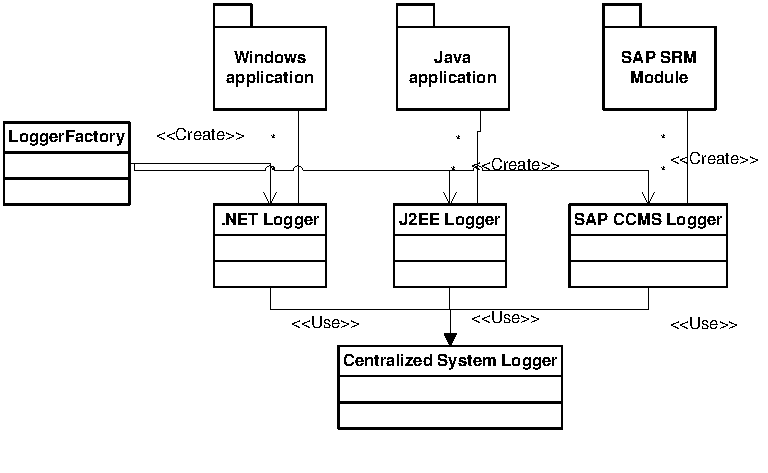
\includegraphics{patterns/systemLoggingDiagram.pdf}
\caption{Main solution structure of BUILT-IN SYSTEM LOGGING}
\label{fig:systemLogging}
\end{figure}

See figure \ref{fig:systemLogging}.

\begin{center}
\ding{118} \ding{118} \ding{118} 
\end{center}

Besides the above mentioned reasons, it is a lot easier to automatically generate incidents from specific defined events from the built-in system log for an IT service management (ITSM) tool. This ITSM tool can be configured to forward the automatically generated incidents directly, without human intervention, to the second line specialists. This way incidents are more easily solved woithout less human in tervention saving valuable time of the system administrators.

Some requirements a good log should met to be valuable are:
\begin{itemize}
	\item Log actions before they happen.
	\item Mind the file size if logs should be copied or archived.
	\item Split messages into different files depending on intended audience/way of using.
\end{itemize}

